\chapter{Metodología}
(Se espera una redacción amplia y detallada la extensión esta determinada por el método seguido por el estudiante)
En este capitulo se presenta el tipo de metodología utilizado en esta tesis, así como las etapas que se seguirán para alcanzar los objetivos establecidos para la investigación.

\section{Tipo de Investigación}
Escribir que tipo de investigación se esta siguiendo.

\section{Métodos de Validación Propuestas}
Cuales serán las métricas utilizadas ?

% Insertando imagen.
  \begin{figure}
  \centering
  \subfloat[]{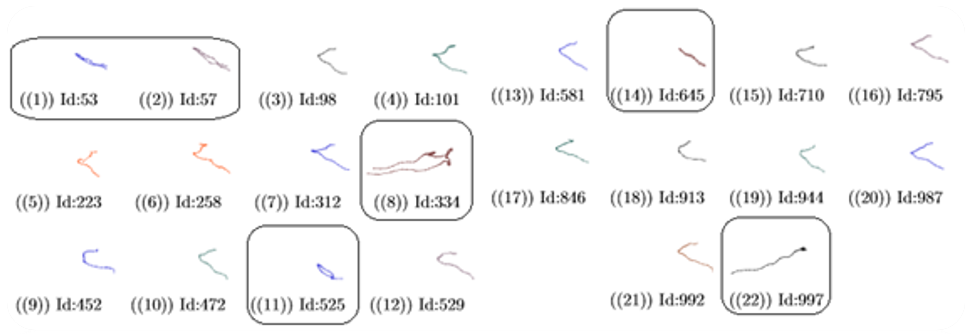
\includegraphics[width=150mm]{graficos/counting.png}}
  \caption[Ejemplo inserción de imagen]
  {Aquí deberas colocar la leyenda o descripción de la imagen.}
 % Nota. Adaptado de Título de la imagen, de Autor de la Imagen, año de publicación de la imagen, Fuente. Tipo de licencia.%
  \label{fig:counting}
  \end{figure}
% Fin insertando imagen

La metodología de investigación hace referencia al conjunto de procedimientos racionales y ordenados utilizados para alcanzar uno o varios objetivos que rigen en una investigación científica, en otras palabras, es el método utilizado para alcanzar los objetivos perseguidos. Se recomienda que el estudiante redacte en forma de párrafos el procedimiento a seguir para la elaboración de investigación.
